\documentclass[12pt]{article}
\usepackage{amsfonts, amssymb, amsmath, amsthm}
\usepackage[margin=1in]{geometry}
\usepackage{tikz}
\usepackage{pgfplots}
\pgfplotsset{compat=1.18}

\title{Explainer: Problem 2 (Rudin 7.7) --- Uniform Convergence vs.\ Derivative Interchange}
\author{}
\date{}

\begin{document}
\maketitle

\section*{What's going on?}
We have $f_n(x) = \frac{x}{1 + nx^2}$. This sequence converges to $f(x) = 0$ for all $x$. The question asks:
\begin{itemize}
    \item Is the convergence uniform? (Yes.)
    \item Can we swap limit and derivative: $f'(x) = \lim f_n'(x)$? (Only for $x \neq 0$.)
\end{itemize}

This is a cautionary tale: \textbf{uniform convergence of $f_n$ does NOT guarantee convergence of $f_n'$}.

\section*{Visualizing $f_n$}

\begin{center}
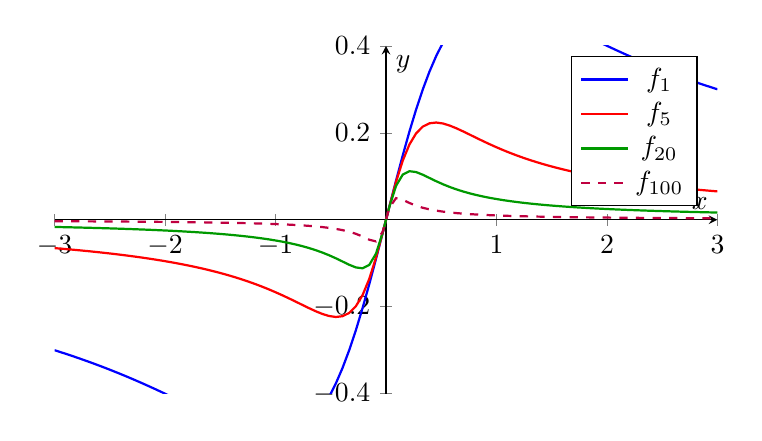
\begin{tikzpicture}
\begin{axis}[
    width=10cm, height=6cm,
    axis lines=middle,
    xlabel={$x$}, ylabel={$y$},
    domain=-3:3, samples=100,
    legend pos=north east,
    ymin=-0.4, ymax=0.4
]
\addplot[blue, thick] {x/(1+1*x^2)};
\addplot[red, thick] {x/(1+5*x^2)};
\addplot[green!60!black, thick] {x/(1+20*x^2)};
\addplot[purple, thick, dashed] {x/(1+100*x^2)};
\legend{$f_1$, $f_5$, $f_{20}$, $f_{100}$}
\end{axis}
\end{tikzpicture}
\end{center}

Each $f_n$ has a bump near the origin that gets \textbf{taller and narrower} as $n$ grows... but not taller than a bound that $\to 0$. The maximum of $|f_n|$ is $\frac{1}{2\sqrt{n}}$ (achieved at $x = \pm 1/\sqrt{n}$), so the sup-norm $\|f_n\|_\infty \to 0$.

\section*{Why uniform convergence holds}

To show $f_n \to 0$ uniformly, we need $\sup_x |f_n(x)| \to 0$.

\textbf{Finding the maximum of $|f_n|$:} By AM--GM or calculus, for $x > 0$:
$$
f_n(x) = \frac{x}{1 + nx^2} = \frac{1}{1/x + nx} \leq \frac{1}{2\sqrt{n}}
$$
since $1/x + nx \geq 2\sqrt{n}$ by AM--GM. Equality when $x = 1/\sqrt{n}$.

So $\|f_n\|_\infty = \frac{1}{2\sqrt{n}} \to 0$. Uniform convergence!

\section*{The derivative story}

Now compute $f_n'(x) = \frac{1 - nx^2}{(1 + nx^2)^2}$.

\textbf{At $x \neq 0$:} As $n \to \infty$, both numerator and denominator are dominated by the $nx^2$ terms, so $f_n'(x) \to 0$. Since $f(x) = 0$, we have $f'(x) = 0 = \lim f_n'(x)$. \checkmark

\textbf{At $x = 0$:} $f_n'(0) = \frac{1 - 0}{(1+0)^2} = 1$ for every $n$. So $\lim f_n'(0) = 1$. But $f(x) = 0$, so $f'(0) = 0 \neq 1$. \ding{55}

\section*{The lesson}

\begin{center}
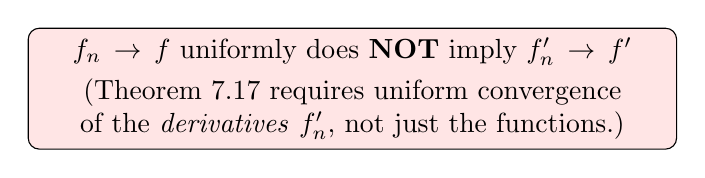
\begin{tikzpicture}[>=stealth]
    \node[draw, rounded corners, fill=red!10, text width=8cm, align=center] at (0,0) {
        $f_n \to f$ uniformly does \textbf{NOT} imply $f_n' \to f'$\\[0.3em]
        (Theorem 7.17 requires uniform convergence of the \emph{derivatives} $f_n'$, not just the functions.)
    };
\end{tikzpicture}
\end{center}

The slopes at $x=0$ stay at $1$ forever even though the functions flatten to $0$ everywhere. The bump gets narrow so fast that its height vanishes, but its slope at the origin never changes.

\end{document}